\documentclass[]{article}
\usepackage{lmodern}
\usepackage{amssymb,amsmath}
\usepackage{ifxetex,ifluatex}
\usepackage{fixltx2e} % provides \textsubscript
\ifnum 0\ifxetex 1\fi\ifluatex 1\fi=0 % if pdftex
  \usepackage[T1]{fontenc}
  \usepackage[utf8]{inputenc}
\else % if luatex or xelatex
  \ifxetex
    \usepackage{mathspec}
  \else
    \usepackage{fontspec}
  \fi
  \defaultfontfeatures{Ligatures=TeX,Scale=MatchLowercase}
\fi
% use upquote if available, for straight quotes in verbatim environments
\IfFileExists{upquote.sty}{\usepackage{upquote}}{}
% use microtype if available
\IfFileExists{microtype.sty}{%
\usepackage{microtype}
\UseMicrotypeSet[protrusion]{basicmath} % disable protrusion for tt fonts
}{}
\usepackage[margin=1in]{geometry}
\usepackage{hyperref}
\hypersetup{unicode=true,
            pdftitle={Home},
            pdfborder={0 0 0},
            breaklinks=true}
\urlstyle{same}  % don't use monospace font for urls
\usepackage{color}
\usepackage{fancyvrb}
\newcommand{\VerbBar}{|}
\newcommand{\VERB}{\Verb[commandchars=\\\{\}]}
\DefineVerbatimEnvironment{Highlighting}{Verbatim}{commandchars=\\\{\}}
% Add ',fontsize=\small' for more characters per line
\usepackage{framed}
\definecolor{shadecolor}{RGB}{248,248,248}
\newenvironment{Shaded}{\begin{snugshade}}{\end{snugshade}}
\newcommand{\KeywordTok}[1]{\textcolor[rgb]{0.13,0.29,0.53}{\textbf{#1}}}
\newcommand{\DataTypeTok}[1]{\textcolor[rgb]{0.13,0.29,0.53}{#1}}
\newcommand{\DecValTok}[1]{\textcolor[rgb]{0.00,0.00,0.81}{#1}}
\newcommand{\BaseNTok}[1]{\textcolor[rgb]{0.00,0.00,0.81}{#1}}
\newcommand{\FloatTok}[1]{\textcolor[rgb]{0.00,0.00,0.81}{#1}}
\newcommand{\ConstantTok}[1]{\textcolor[rgb]{0.00,0.00,0.00}{#1}}
\newcommand{\CharTok}[1]{\textcolor[rgb]{0.31,0.60,0.02}{#1}}
\newcommand{\SpecialCharTok}[1]{\textcolor[rgb]{0.00,0.00,0.00}{#1}}
\newcommand{\StringTok}[1]{\textcolor[rgb]{0.31,0.60,0.02}{#1}}
\newcommand{\VerbatimStringTok}[1]{\textcolor[rgb]{0.31,0.60,0.02}{#1}}
\newcommand{\SpecialStringTok}[1]{\textcolor[rgb]{0.31,0.60,0.02}{#1}}
\newcommand{\ImportTok}[1]{#1}
\newcommand{\CommentTok}[1]{\textcolor[rgb]{0.56,0.35,0.01}{\textit{#1}}}
\newcommand{\DocumentationTok}[1]{\textcolor[rgb]{0.56,0.35,0.01}{\textbf{\textit{#1}}}}
\newcommand{\AnnotationTok}[1]{\textcolor[rgb]{0.56,0.35,0.01}{\textbf{\textit{#1}}}}
\newcommand{\CommentVarTok}[1]{\textcolor[rgb]{0.56,0.35,0.01}{\textbf{\textit{#1}}}}
\newcommand{\OtherTok}[1]{\textcolor[rgb]{0.56,0.35,0.01}{#1}}
\newcommand{\FunctionTok}[1]{\textcolor[rgb]{0.00,0.00,0.00}{#1}}
\newcommand{\VariableTok}[1]{\textcolor[rgb]{0.00,0.00,0.00}{#1}}
\newcommand{\ControlFlowTok}[1]{\textcolor[rgb]{0.13,0.29,0.53}{\textbf{#1}}}
\newcommand{\OperatorTok}[1]{\textcolor[rgb]{0.81,0.36,0.00}{\textbf{#1}}}
\newcommand{\BuiltInTok}[1]{#1}
\newcommand{\ExtensionTok}[1]{#1}
\newcommand{\PreprocessorTok}[1]{\textcolor[rgb]{0.56,0.35,0.01}{\textit{#1}}}
\newcommand{\AttributeTok}[1]{\textcolor[rgb]{0.77,0.63,0.00}{#1}}
\newcommand{\RegionMarkerTok}[1]{#1}
\newcommand{\InformationTok}[1]{\textcolor[rgb]{0.56,0.35,0.01}{\textbf{\textit{#1}}}}
\newcommand{\WarningTok}[1]{\textcolor[rgb]{0.56,0.35,0.01}{\textbf{\textit{#1}}}}
\newcommand{\AlertTok}[1]{\textcolor[rgb]{0.94,0.16,0.16}{#1}}
\newcommand{\ErrorTok}[1]{\textcolor[rgb]{0.64,0.00,0.00}{\textbf{#1}}}
\newcommand{\NormalTok}[1]{#1}
\usepackage{graphicx,grffile}
\makeatletter
\def\maxwidth{\ifdim\Gin@nat@width>\linewidth\linewidth\else\Gin@nat@width\fi}
\def\maxheight{\ifdim\Gin@nat@height>\textheight\textheight\else\Gin@nat@height\fi}
\makeatother
% Scale images if necessary, so that they will not overflow the page
% margins by default, and it is still possible to overwrite the defaults
% using explicit options in \includegraphics[width, height, ...]{}
\setkeys{Gin}{width=\maxwidth,height=\maxheight,keepaspectratio}
\IfFileExists{parskip.sty}{%
\usepackage{parskip}
}{% else
\setlength{\parindent}{0pt}
\setlength{\parskip}{6pt plus 2pt minus 1pt}
}
\setlength{\emergencystretch}{3em}  % prevent overfull lines
\providecommand{\tightlist}{%
  \setlength{\itemsep}{0pt}\setlength{\parskip}{0pt}}
\setcounter{secnumdepth}{0}
% Redefines (sub)paragraphs to behave more like sections
\ifx\paragraph\undefined\else
\let\oldparagraph\paragraph
\renewcommand{\paragraph}[1]{\oldparagraph{#1}\mbox{}}
\fi
\ifx\subparagraph\undefined\else
\let\oldsubparagraph\subparagraph
\renewcommand{\subparagraph}[1]{\oldsubparagraph{#1}\mbox{}}
\fi

%%% Use protect on footnotes to avoid problems with footnotes in titles
\let\rmarkdownfootnote\footnote%
\def\footnote{\protect\rmarkdownfootnote}

%%% Change title format to be more compact
\usepackage{titling}

% Create subtitle command for use in maketitle
\providecommand{\subtitle}[1]{
  \posttitle{
    \begin{center}\large#1\end{center}
    }
}

\setlength{\droptitle}{-2em}

  \title{Home}
    \pretitle{\vspace{\droptitle}\centering\huge}
  \posttitle{\par}
    \author{}
    \preauthor{}\postauthor{}
    \date{}
    \predate{}\postdate{}
  

\begin{document}
\maketitle

This is an analysis to estimate population trends for Canada Warbler
using the data from the North American Breeding Bird Survey (BBS) from
2002 through 2012. The primary purpose of this analysis is to compare
trends estimated here with trends for the same time-period estimated
from the Boreal Avian Modeling project (BAM). I will be using the
package bbsBayes to estimate the trends for the standard CWS analytical
strata. I will select the ``slope'' model for the trends.

\begin{Shaded}
\begin{Highlighting}[]
\KeywordTok{library}\NormalTok{(bbsBayes)}
\KeywordTok{library}\NormalTok{(ggplot2)}
\end{Highlighting}
\end{Shaded}

Loading the BBS data, data-version 2018 Pardieck, K.L., D.J. Ziolkowski
Jr., M. Lutmerding, V. Aponte and M-A.R. Hudson. 2019. North American
Breeding Bird Survey Dataset 1966 - 2018, version 2018.0. U.S.
Geological Survey, Patuxent Wildlife Research Center.
\url{https://doi.org/10.5066/P9HE8XYJ}.

The user must have already downloaded the BBS data

Stratify the data using the standard CWS strata (BCR by province
intersections)

\begin{Shaded}
\begin{Highlighting}[]
\NormalTok{bbs_strat =}\StringTok{ }\KeywordTok{stratify}\NormalTok{(}\DataTypeTok{by =} \StringTok{"bbs_cws"}\NormalTok{,}\DataTypeTok{quiet =}\NormalTok{ T)}
\end{Highlighting}
\end{Shaded}

Prepare the data for jags, selecting the start and end years, as well as
the species and model

\begin{Shaded}
\begin{Highlighting}[]
\NormalTok{bbs_data =}\StringTok{ }\KeywordTok{prepare_jags_data}\NormalTok{(}\DataTypeTok{strat_data =}\NormalTok{ bbs_strat,}
                             \DataTypeTok{species_to_run =} \StringTok{"Canada Warbler"}\NormalTok{,}
                             \DataTypeTok{model =} \StringTok{"slope"}\NormalTok{,}
                             \DataTypeTok{min_year =} \DecValTok{2002}\NormalTok{,}
                             \DataTypeTok{max_year =} \DecValTok{2012}\NormalTok{,}
                             \DataTypeTok{quiet =}\NormalTok{ T)}
\end{Highlighting}
\end{Shaded}

Run the model in jags, tracking the random and fixed slope effects as
well as the annual indices

\begin{Shaded}
\begin{Highlighting}[]
\NormalTok{mod =}\StringTok{ }\KeywordTok{run_model}\NormalTok{(}\DataTypeTok{jags_data =}\NormalTok{ bbs_data,}
                \DataTypeTok{parameters_to_save =} \KeywordTok{c}\NormalTok{(}\StringTok{"n"}\NormalTok{,}\StringTok{"beta"}\NormalTok{,}\StringTok{"BETA"}\NormalTok{),}
                \DataTypeTok{n_adapt =} \DecValTok{1000}\NormalTok{,}
                \DataTypeTok{n_burnin =} \DecValTok{30000}\NormalTok{,}
                \DataTypeTok{n_iter =} \DecValTok{80000}\NormalTok{,}
                \DataTypeTok{n_thin =} \DecValTok{10}\NormalTok{,}
                \DataTypeTok{parallel =}\NormalTok{ T)}
\end{Highlighting}
\end{Shaded}

\begin{verbatim}
## 
## Processing function input....... 
## 
## Done. 
##  
## Beginning parallel processing using 3 cores. Console output will be suppressed.
## 
## Parallel processing completed.
## 
## Calculating statistics....... 
## 
## Done.
\end{verbatim}

calculate indices

\begin{Shaded}
\begin{Highlighting}[]
\NormalTok{ind.s =}\StringTok{ }\KeywordTok{generate_strata_indices}\NormalTok{(mod)}
\NormalTok{trends.s =}\StringTok{ }\KeywordTok{generate_strata_trends}\NormalTok{(ind.s,}\DataTypeTok{slope =}\NormalTok{ T)}


\NormalTok{ind.c =}\StringTok{ }\KeywordTok{generate_cont_indices}\NormalTok{(mod)}
\NormalTok{trends.c =}\StringTok{ }\KeywordTok{generate_cont_trend}\NormalTok{(ind.c,}\DataTypeTok{slope =}\NormalTok{ T)}

\NormalTok{trendsout =}\StringTok{ }\KeywordTok{rbind}\NormalTok{(trends.c,trends.s)}
\KeywordTok{write.csv}\NormalTok{(trendsout,}\StringTok{"all CAWA stratum and continental trends 2002 2012.csv"}\NormalTok{)}


\CommentTok{#}
\KeywordTok{source}\NormalTok{(}\StringTok{"C:/Users/smithac/Documents/GitHub/temp/generate-regional-indices.R"}\NormalTok{)}
\KeywordTok{source}\NormalTok{(}\StringTok{"C:/Users/smithac/Documents/GitHub/temp/generate-regional-trends.R"}\NormalTok{)}

\NormalTok{ind.reg =}\StringTok{ }\KeywordTok{generate_regional_indices}\NormalTok{(mod)}
\NormalTok{trends.reg =}\StringTok{ }\KeywordTok{generate_regional_trend}\NormalTok{(ind.reg)}

\KeywordTok{write.csv}\NormalTok{(trends.reg,}\StringTok{"all CAWA regional trends 2002 2012.csv"}\NormalTok{)}
\end{Highlighting}
\end{Shaded}

graph the indices and map the trends

\begin{Shaded}
\begin{Highlighting}[]
\KeywordTok{generate_map}\NormalTok{(}\DataTypeTok{trend =}\NormalTok{ trends.s, }\DataTypeTok{stratify_by =} \StringTok{"bbs_cws"}\NormalTok{)}
\end{Highlighting}
\end{Shaded}

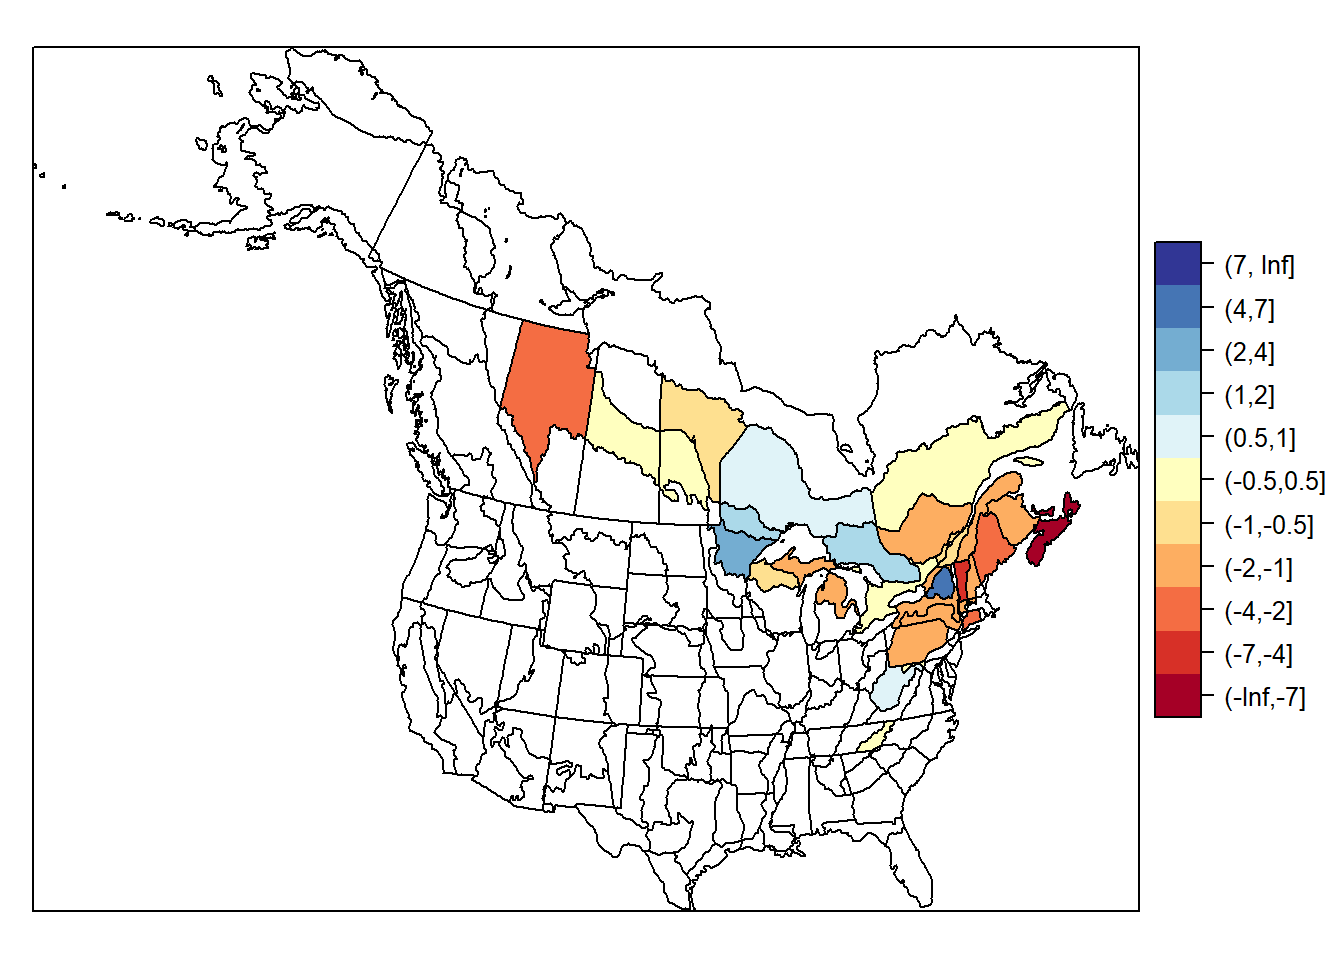
\includegraphics{index_files/figure-latex/unnamed-chunk-7-1.pdf}

\begin{Shaded}
\begin{Highlighting}[]
\KeywordTok{plot_cont_indices}\NormalTok{(}\DataTypeTok{indices_list =}\NormalTok{ ind.c,}\DataTypeTok{add_observed_means =}\NormalTok{ T)}
\end{Highlighting}
\end{Shaded}

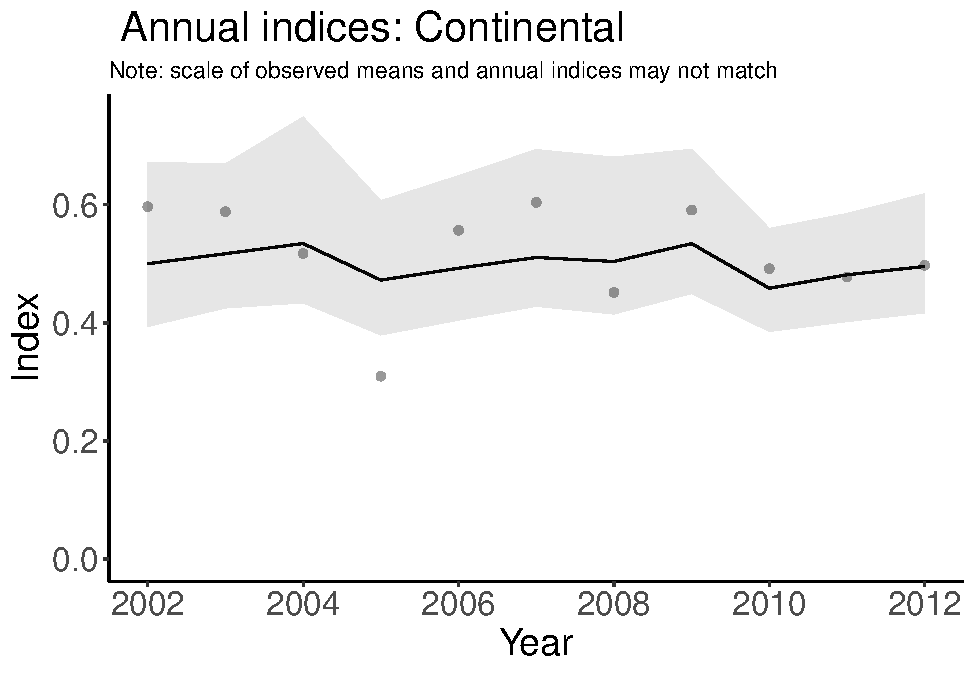
\includegraphics{index_files/figure-latex/unnamed-chunk-7-2.pdf}

\begin{Shaded}
\begin{Highlighting}[]
\NormalTok{tp =}\StringTok{ }\KeywordTok{plot_strata_indices}\NormalTok{(}\DataTypeTok{indices_list =}\NormalTok{ ind.s,}\DataTypeTok{add_observed_means =}\NormalTok{ T)}
\KeywordTok{print}\NormalTok{(tp)}
\end{Highlighting}
\end{Shaded}

\begin{verbatim}
## $CA_AB_6
\end{verbatim}

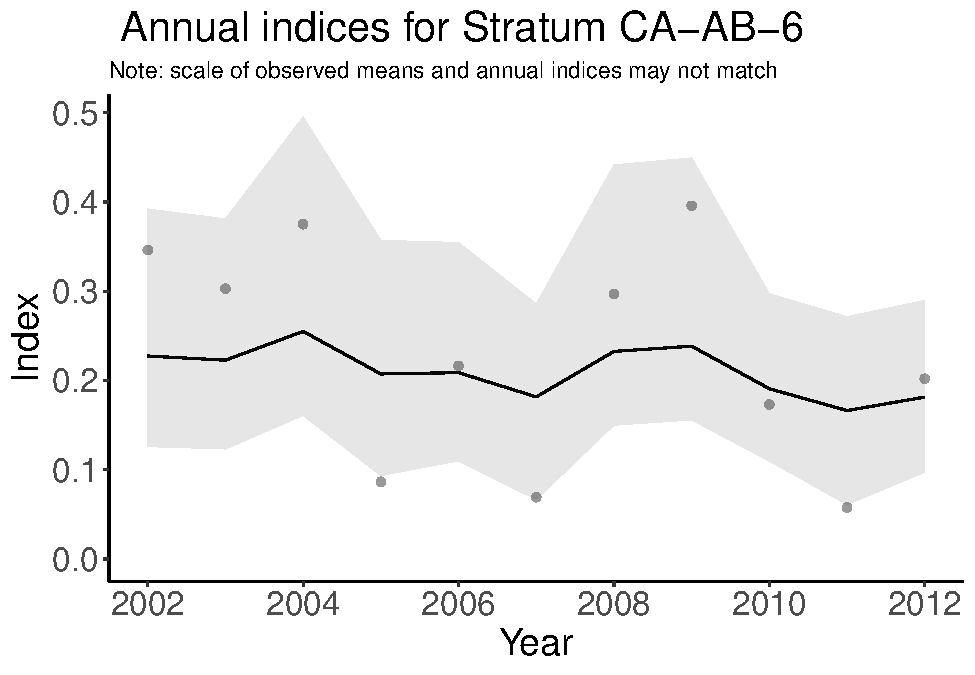
\includegraphics{index_files/figure-latex/unnamed-chunk-7-3.pdf}

\begin{verbatim}
## 
## $CA_MB_6
\end{verbatim}

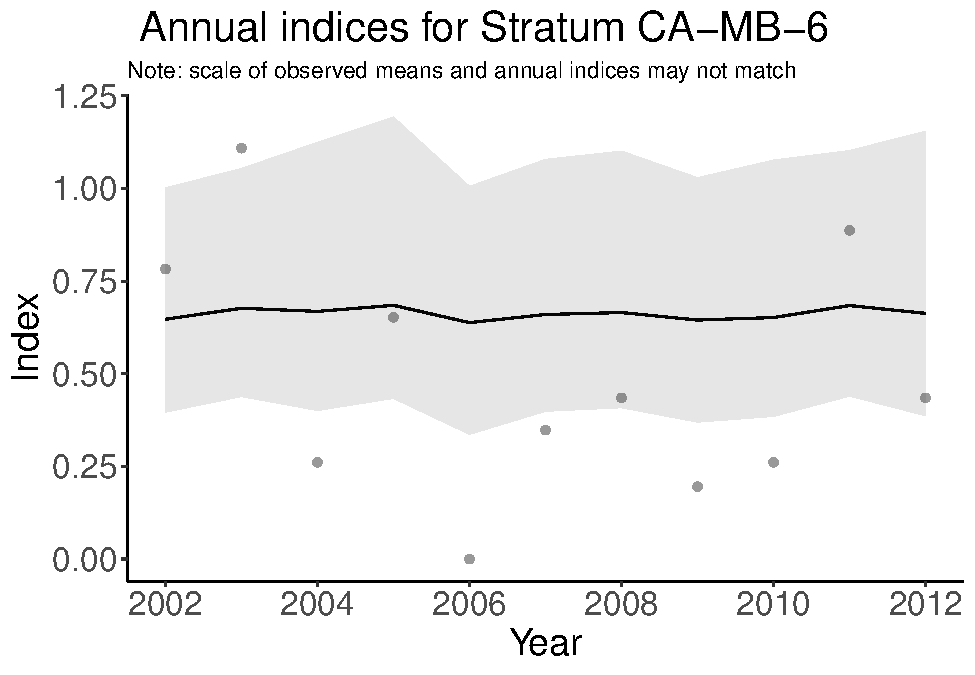
\includegraphics{index_files/figure-latex/unnamed-chunk-7-4.pdf}

\begin{verbatim}
## 
## $CA_MB_8
\end{verbatim}

\begin{verbatim}
## Warning: Removed 1 rows containing missing values (geom_point).
\end{verbatim}

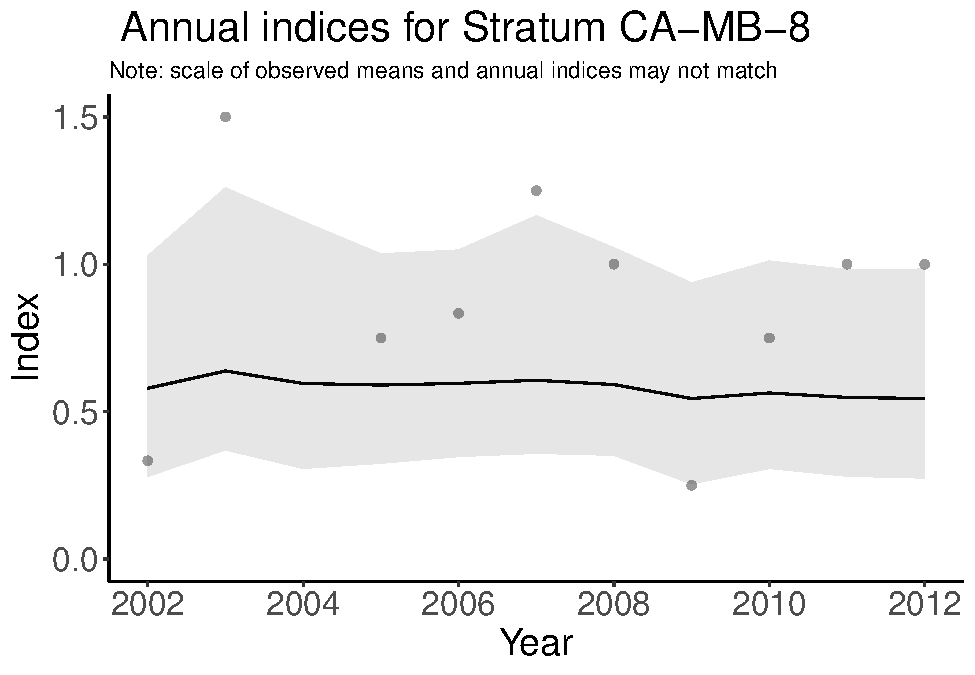
\includegraphics{index_files/figure-latex/unnamed-chunk-7-5.pdf}

\begin{verbatim}
## 
## $CA_NB_14
\end{verbatim}

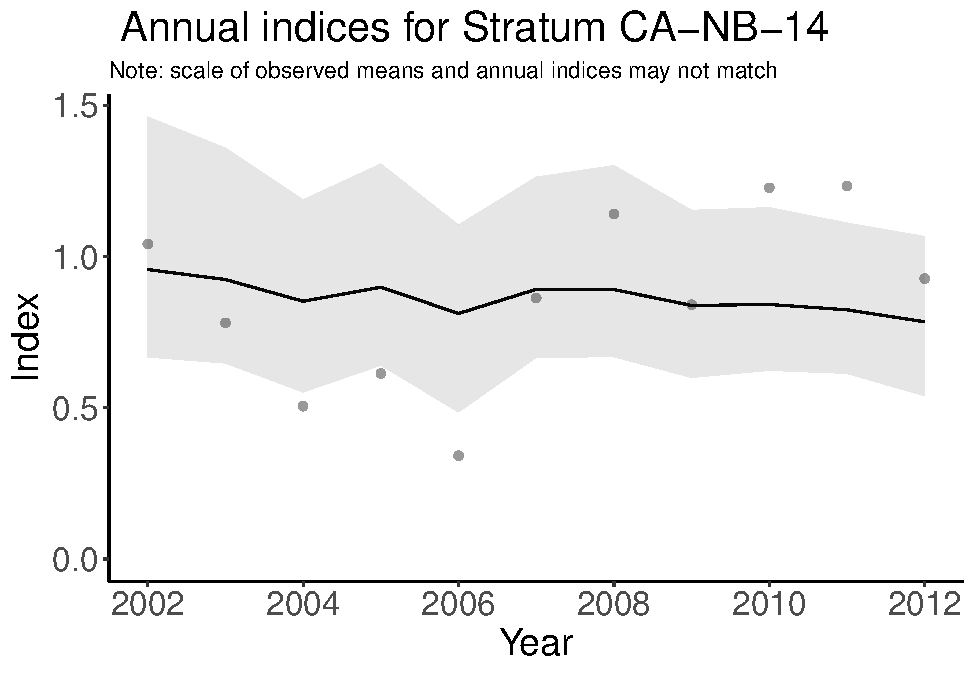
\includegraphics{index_files/figure-latex/unnamed-chunk-7-6.pdf}

\begin{verbatim}
## 
## $CA_NSPE_14
\end{verbatim}

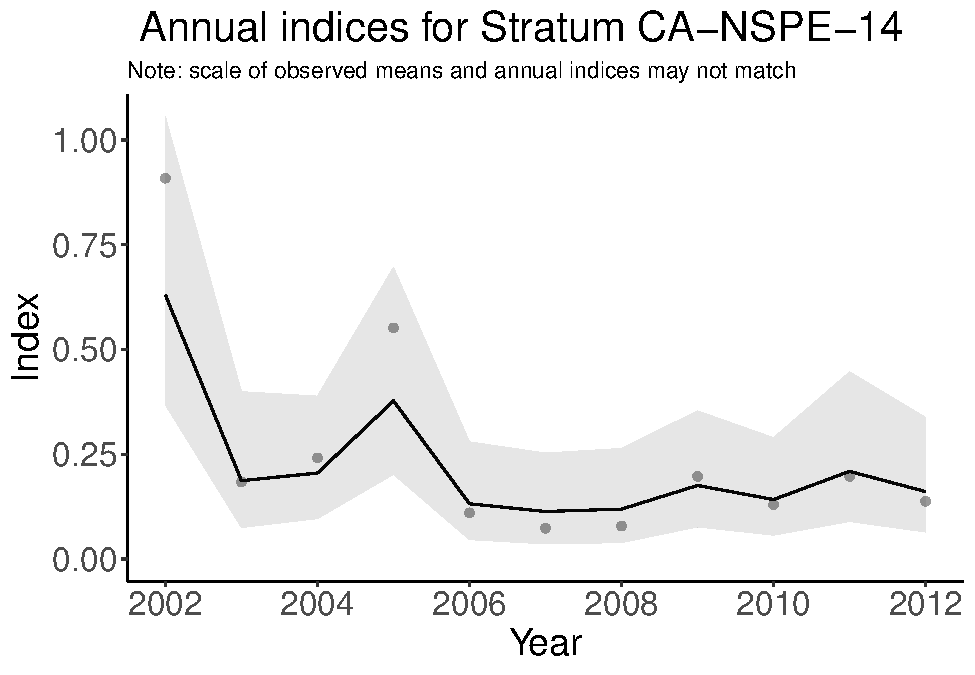
\includegraphics{index_files/figure-latex/unnamed-chunk-7-7.pdf}

\begin{verbatim}
## 
## $CA_ON_12
\end{verbatim}

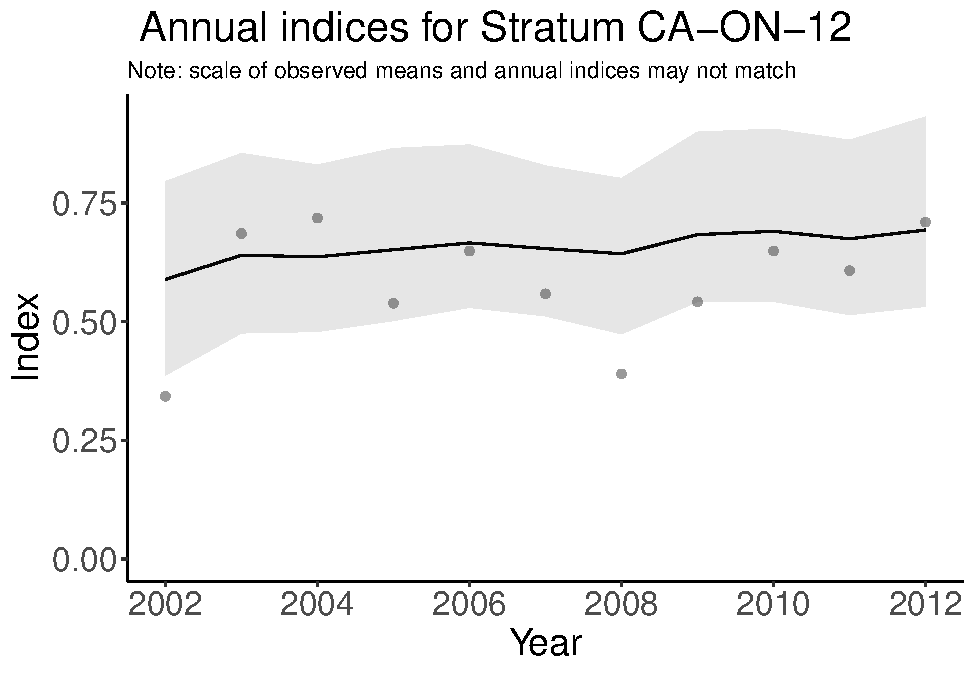
\includegraphics{index_files/figure-latex/unnamed-chunk-7-8.pdf}

\begin{verbatim}
## 
## $CA_ON_13
\end{verbatim}

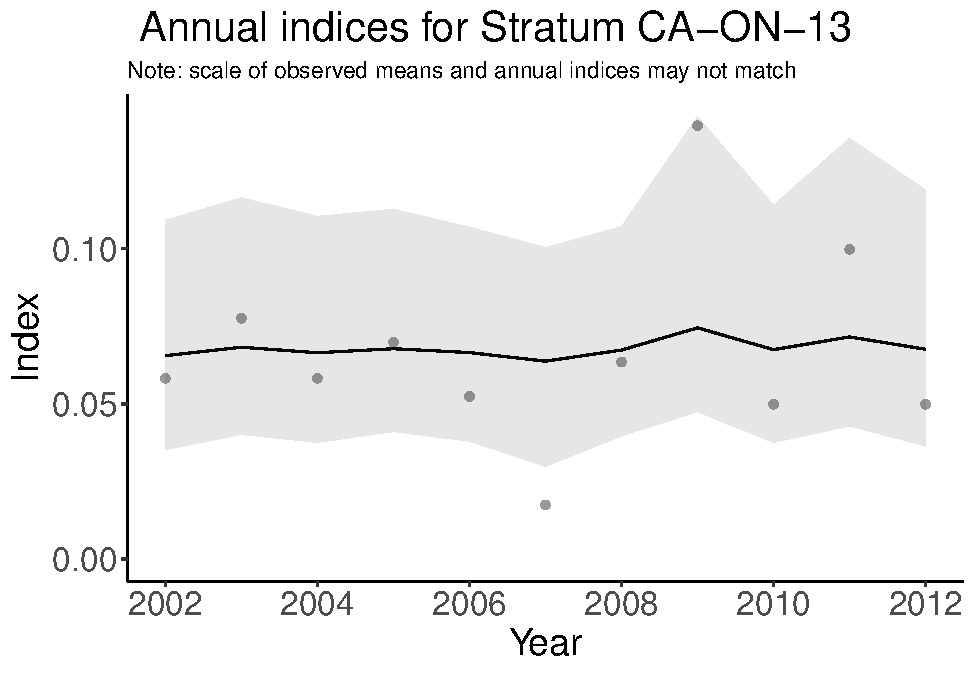
\includegraphics{index_files/figure-latex/unnamed-chunk-7-9.pdf}

\begin{verbatim}
## 
## $CA_ON_8
\end{verbatim}

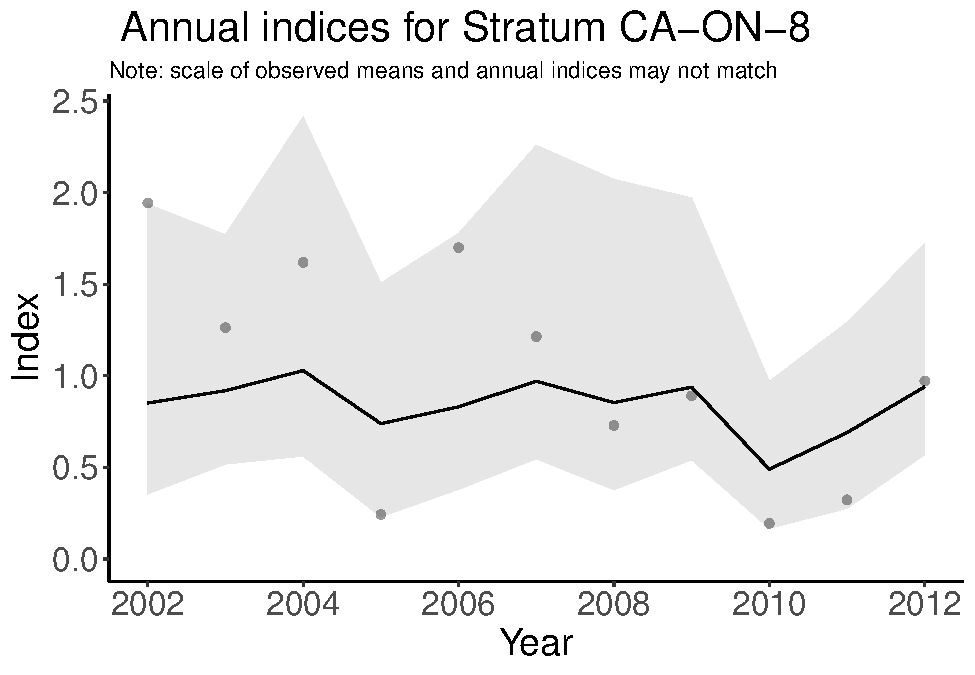
\includegraphics{index_files/figure-latex/unnamed-chunk-7-10.pdf}

\begin{verbatim}
## 
## $CA_QC_12
\end{verbatim}

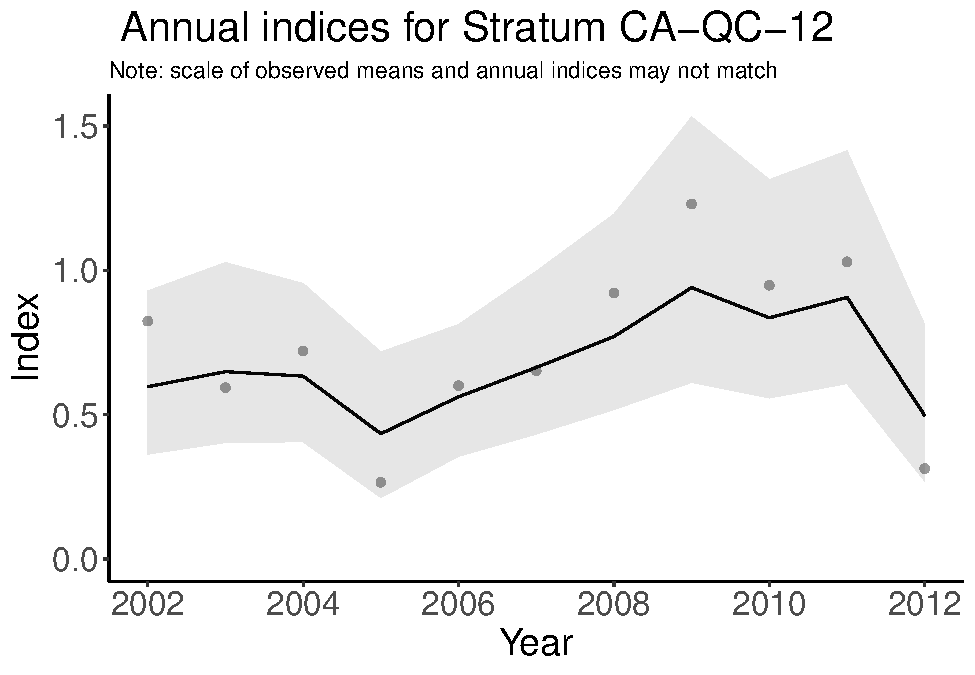
\includegraphics{index_files/figure-latex/unnamed-chunk-7-11.pdf}

\begin{verbatim}
## 
## $CA_QC_13
\end{verbatim}

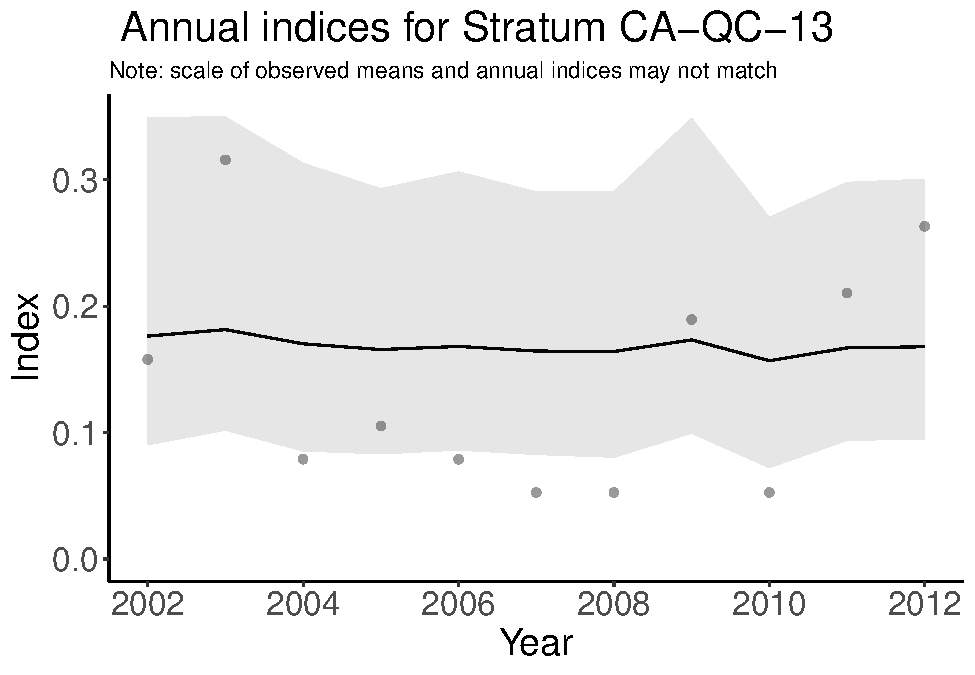
\includegraphics{index_files/figure-latex/unnamed-chunk-7-12.pdf}

\begin{verbatim}
## 
## $CA_QC_14
\end{verbatim}

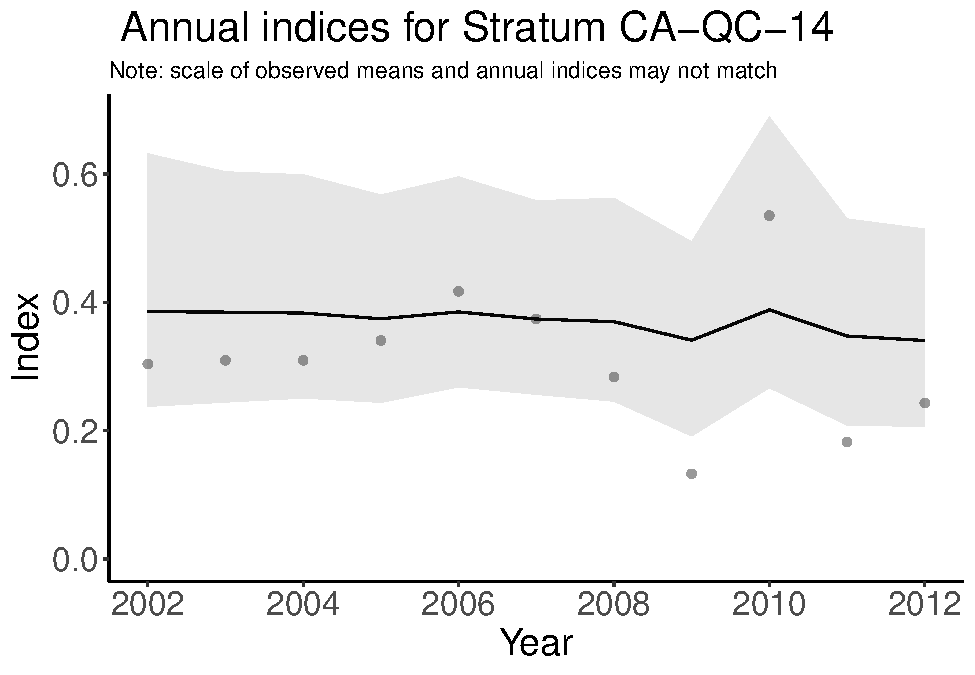
\includegraphics{index_files/figure-latex/unnamed-chunk-7-13.pdf}

\begin{verbatim}
## 
## $CA_QC_8
\end{verbatim}

\begin{verbatim}
## Warning: Removed 4 rows containing missing values (geom_point).
\end{verbatim}

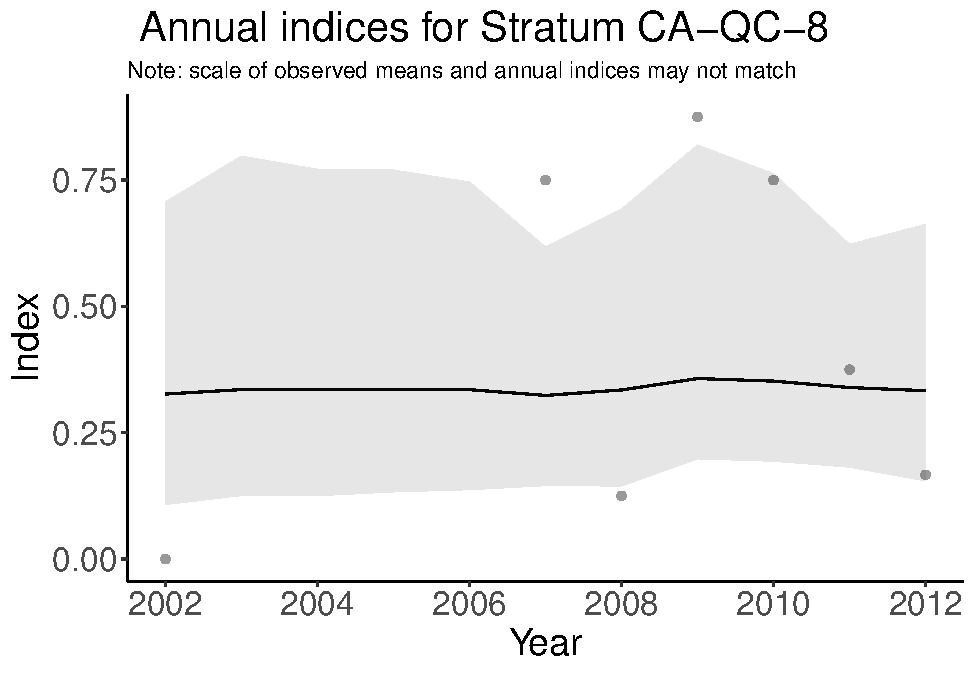
\includegraphics{index_files/figure-latex/unnamed-chunk-7-14.pdf}

\begin{verbatim}
## 
## $CA_SK_6
\end{verbatim}

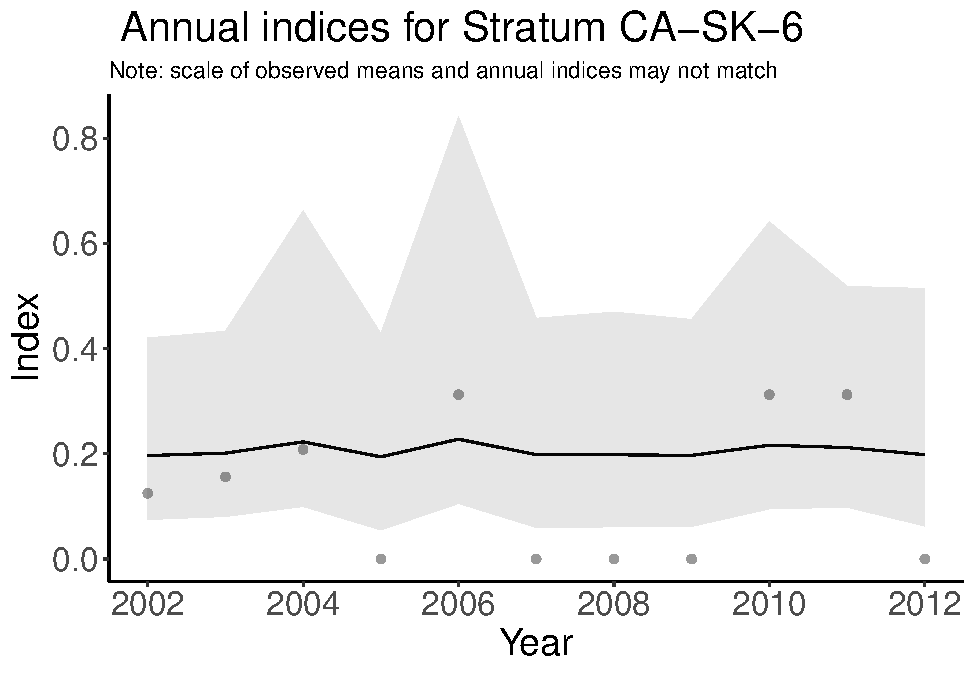
\includegraphics{index_files/figure-latex/unnamed-chunk-7-15.pdf}

\begin{verbatim}
## 
## $US_CT_30
\end{verbatim}

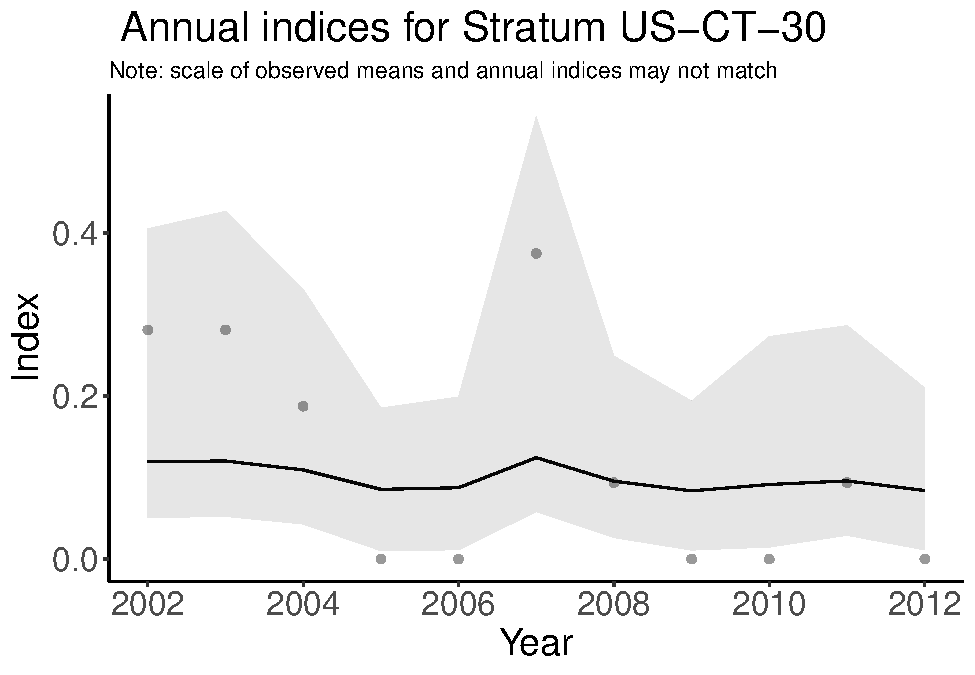
\includegraphics{index_files/figure-latex/unnamed-chunk-7-16.pdf}

\begin{verbatim}
## 
## $US_MA_14
\end{verbatim}

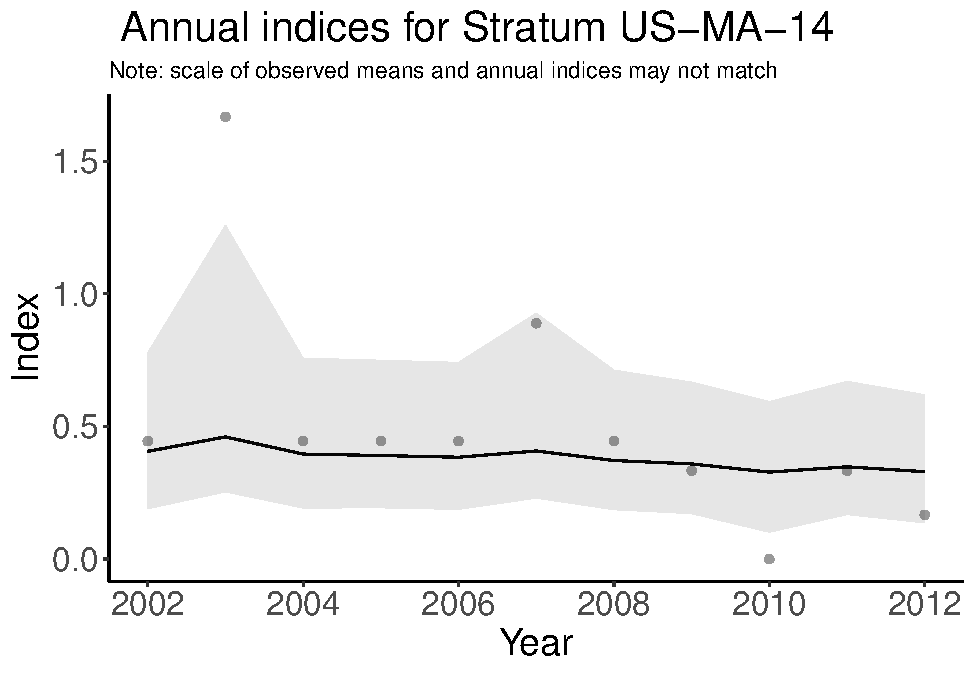
\includegraphics{index_files/figure-latex/unnamed-chunk-7-17.pdf}

\begin{verbatim}
## 
## $US_MD_28
\end{verbatim}

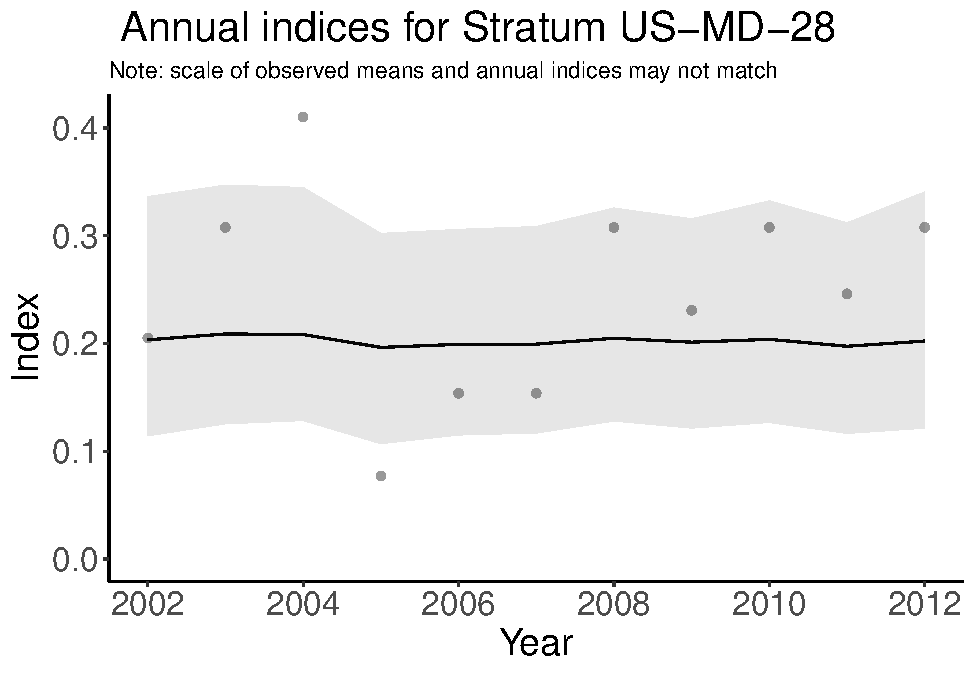
\includegraphics{index_files/figure-latex/unnamed-chunk-7-18.pdf}

\begin{verbatim}
## 
## $US_ME_14
\end{verbatim}

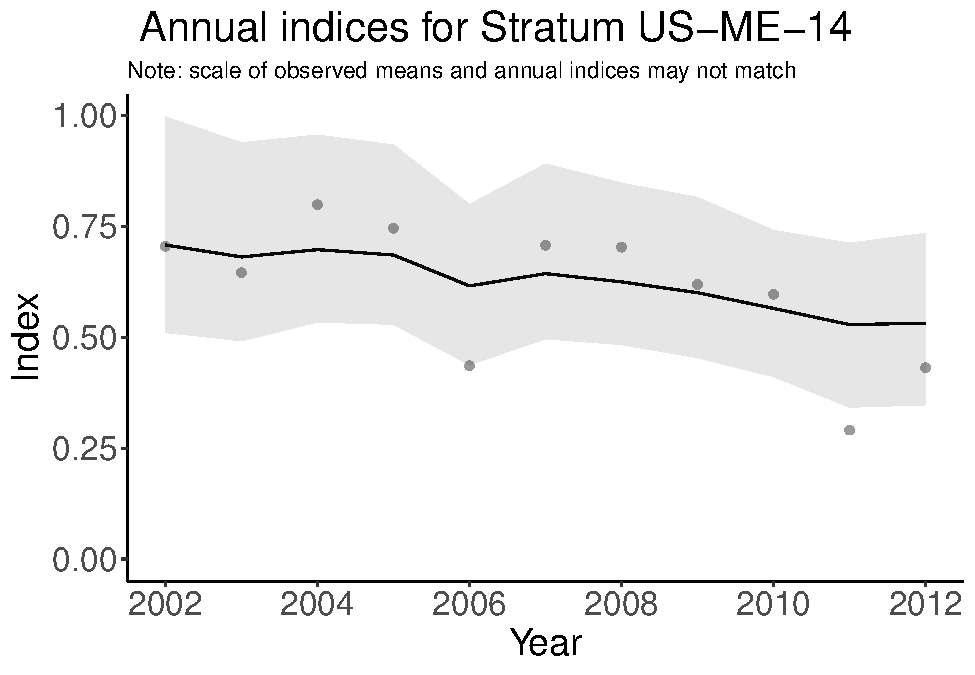
\includegraphics{index_files/figure-latex/unnamed-chunk-7-19.pdf}

\begin{verbatim}
## 
## $US_MI_12
\end{verbatim}

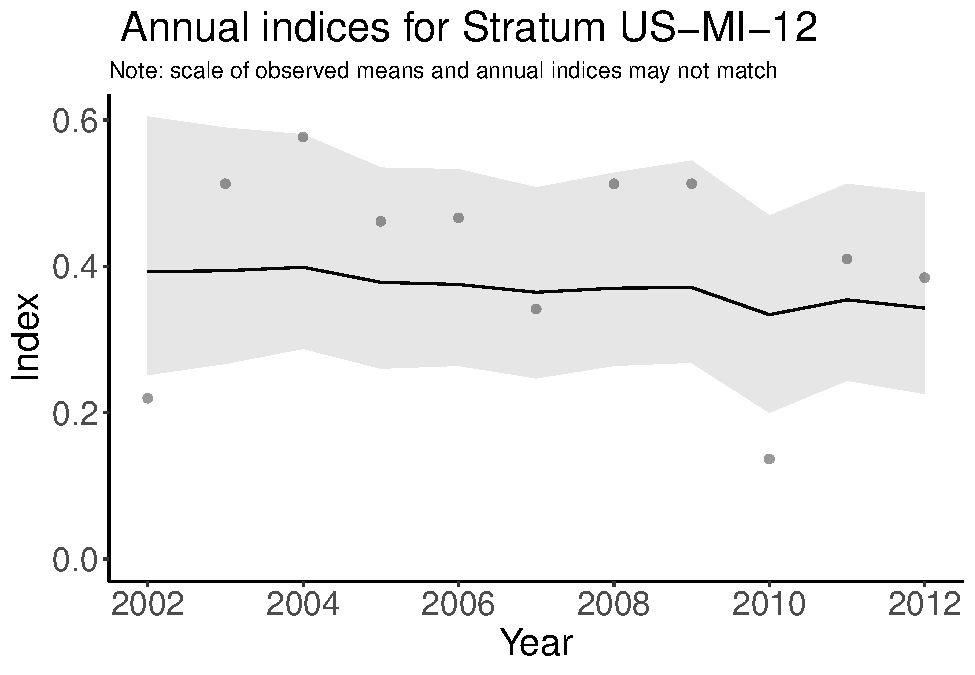
\includegraphics{index_files/figure-latex/unnamed-chunk-7-20.pdf}

\begin{verbatim}
## 
## $US_MN_12
\end{verbatim}

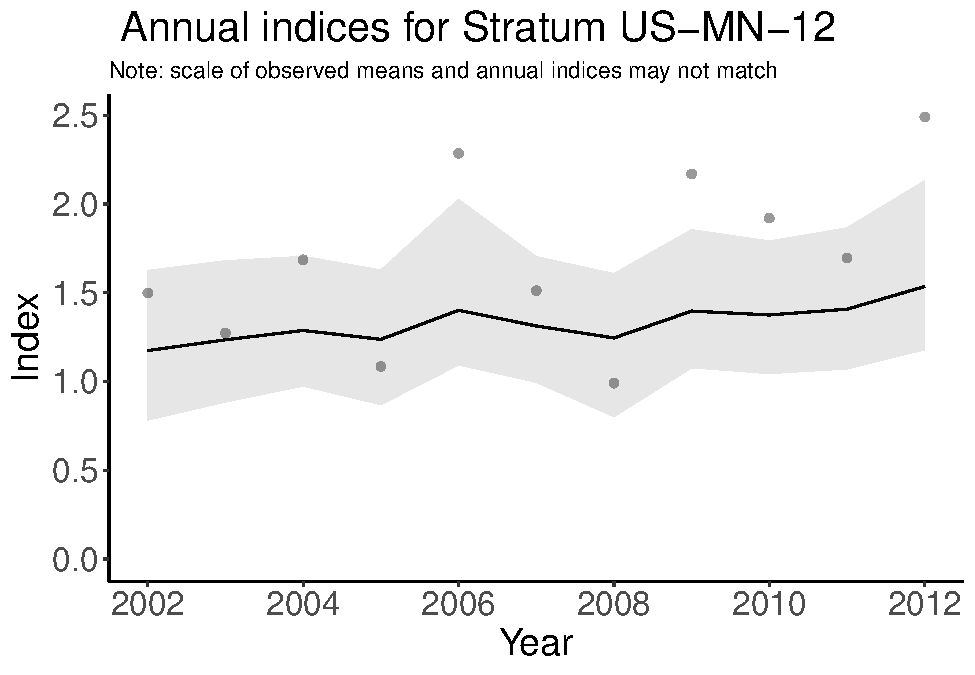
\includegraphics{index_files/figure-latex/unnamed-chunk-7-21.pdf}

\begin{verbatim}
## 
## $US_NC_28
\end{verbatim}

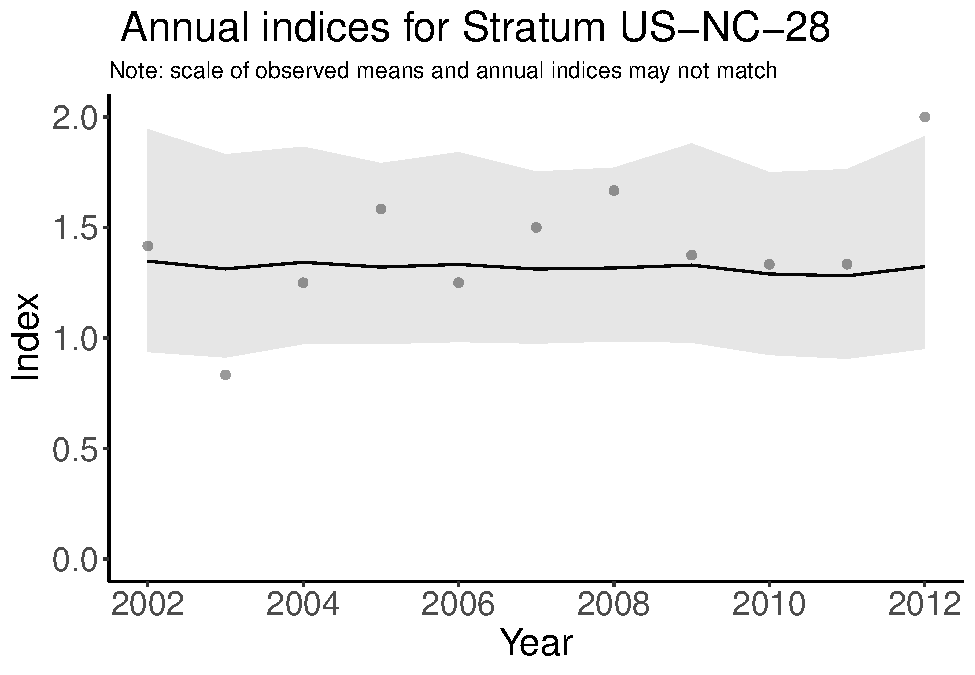
\includegraphics{index_files/figure-latex/unnamed-chunk-7-22.pdf}

\begin{verbatim}
## 
## $US_NH_14
\end{verbatim}

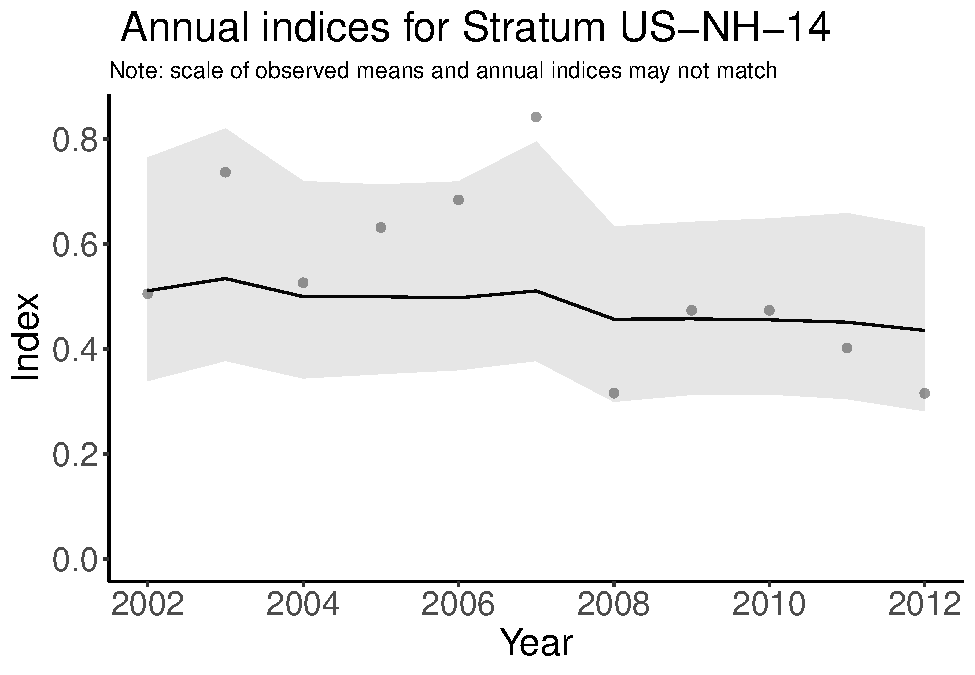
\includegraphics{index_files/figure-latex/unnamed-chunk-7-23.pdf}

\begin{verbatim}
## 
## $US_NY_13
\end{verbatim}

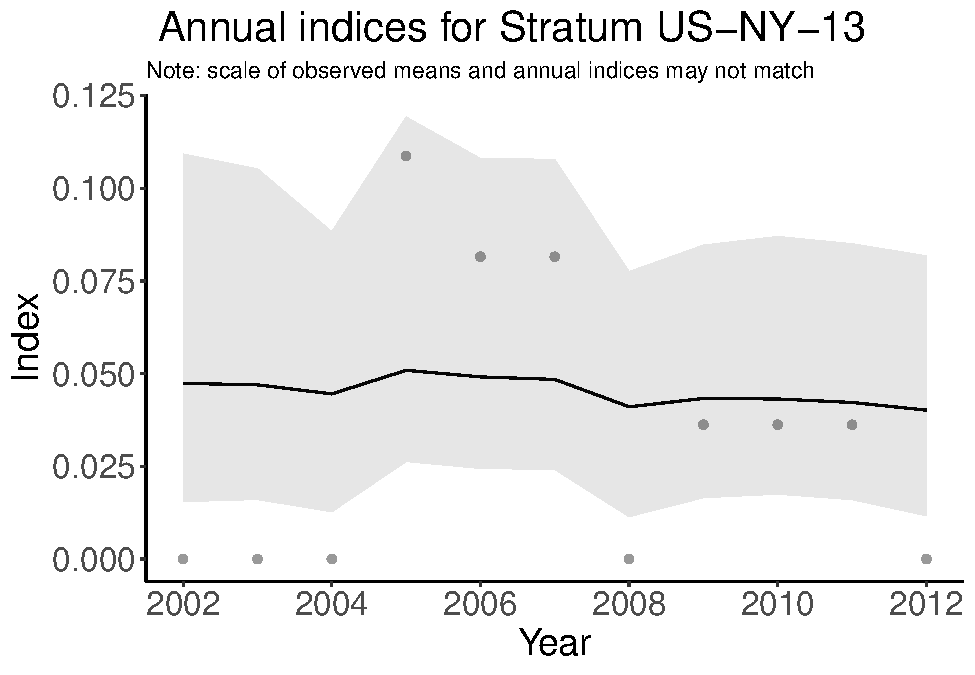
\includegraphics{index_files/figure-latex/unnamed-chunk-7-24.pdf}

\begin{verbatim}
## 
## $US_NY_14
\end{verbatim}

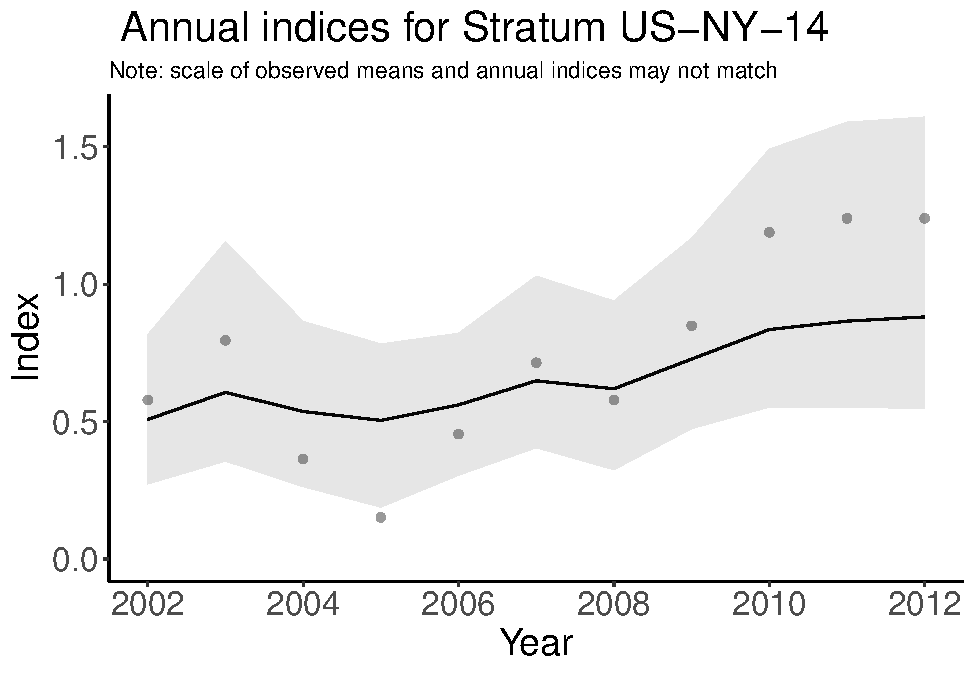
\includegraphics{index_files/figure-latex/unnamed-chunk-7-25.pdf}

\begin{verbatim}
## 
## $US_NY_28
\end{verbatim}

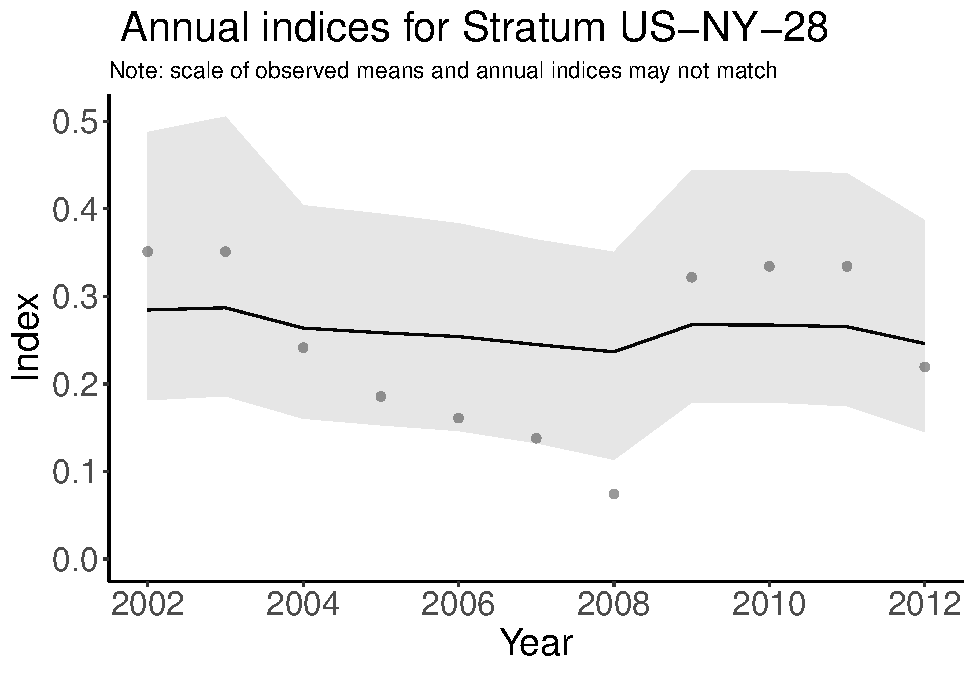
\includegraphics{index_files/figure-latex/unnamed-chunk-7-26.pdf}

\begin{verbatim}
## 
## $US_PA_28
\end{verbatim}

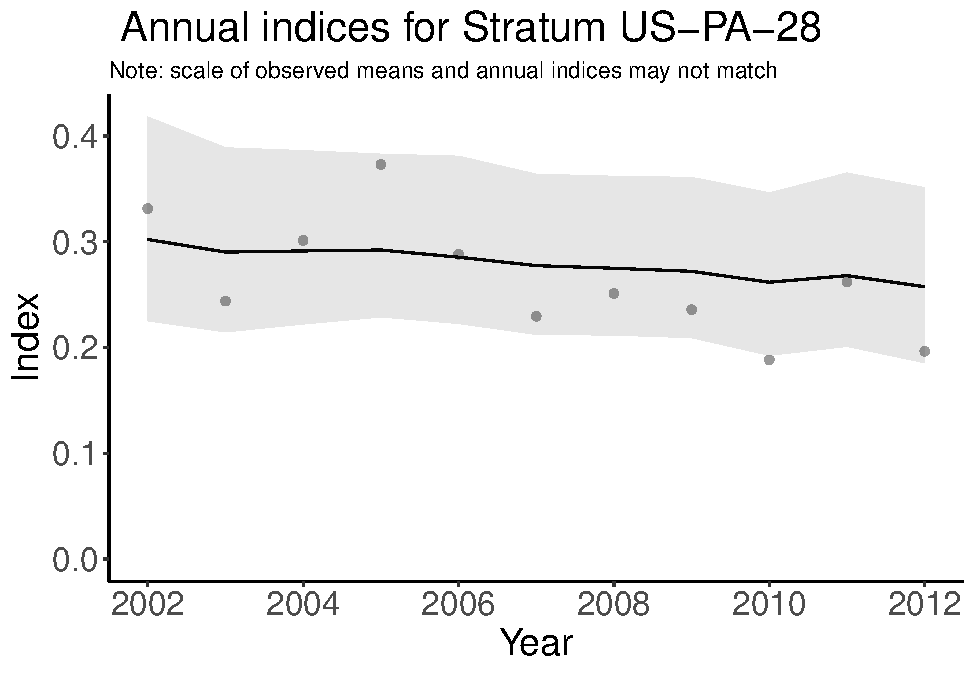
\includegraphics{index_files/figure-latex/unnamed-chunk-7-27.pdf}

\begin{verbatim}
## 
## $US_VT_14
\end{verbatim}

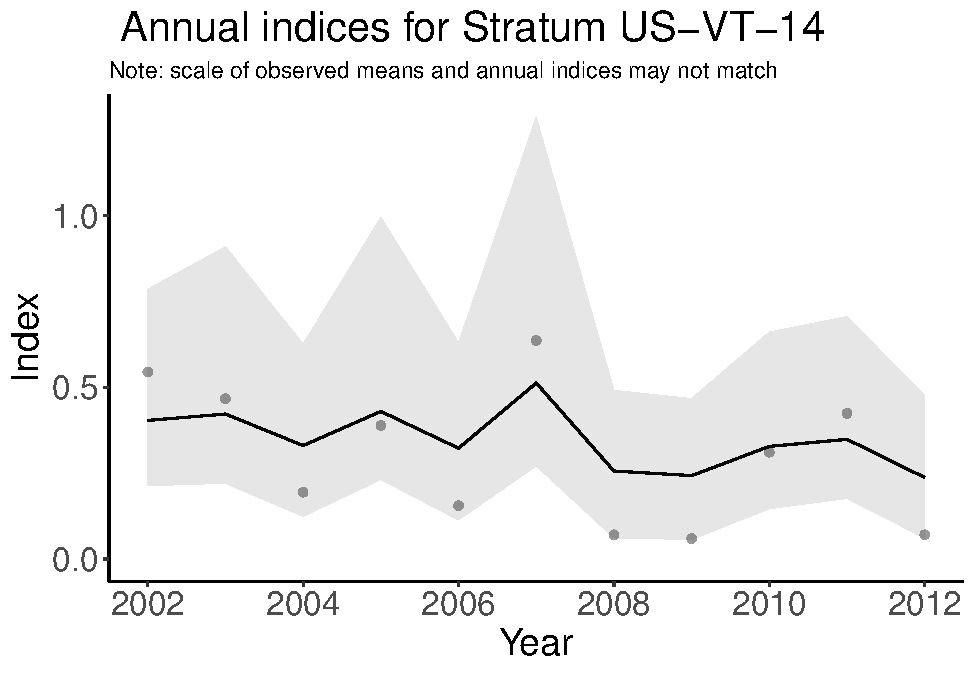
\includegraphics{index_files/figure-latex/unnamed-chunk-7-28.pdf}

\begin{verbatim}
## 
## $US_WI_12
\end{verbatim}

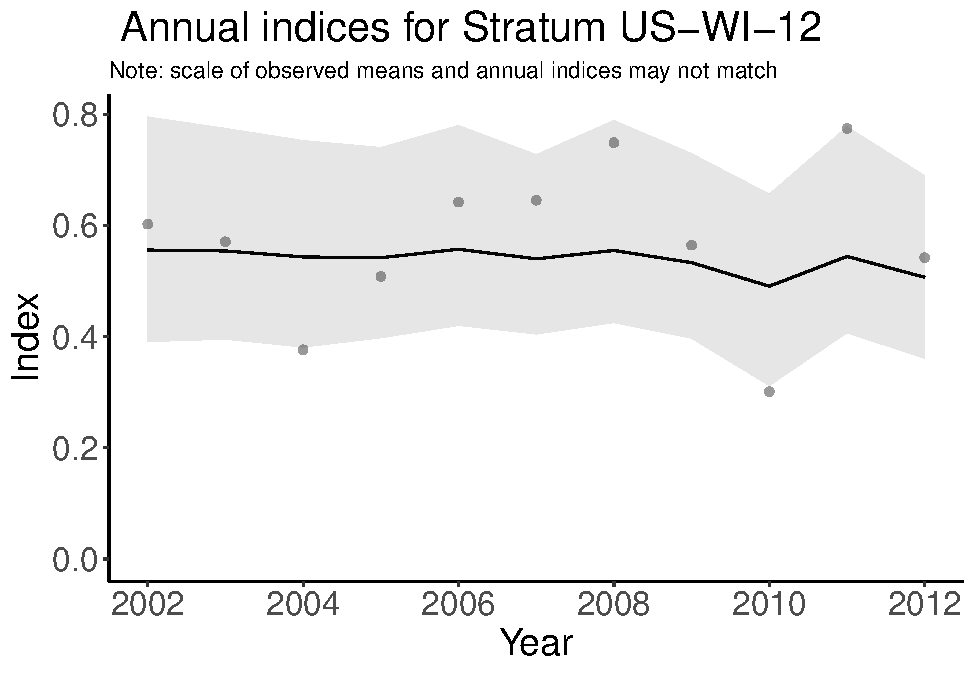
\includegraphics{index_files/figure-latex/unnamed-chunk-7-29.pdf}

\begin{verbatim}
## 
## $US_WV_28
\end{verbatim}

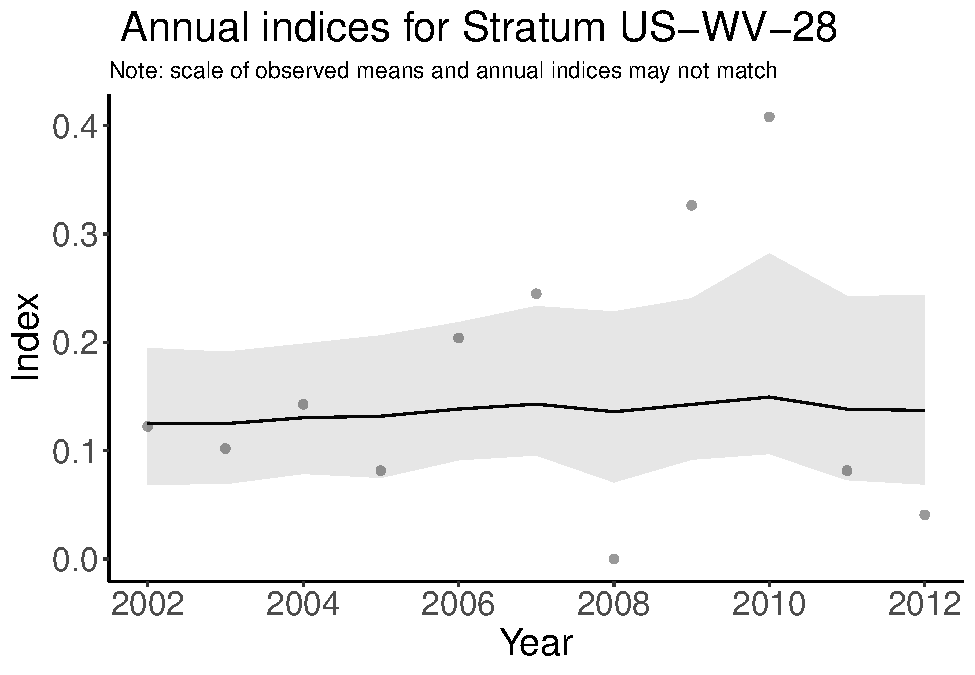
\includegraphics{index_files/figure-latex/unnamed-chunk-7-30.pdf}

\begin{Shaded}
\begin{Highlighting}[]
\NormalTok{tp2 =}\StringTok{ }\KeywordTok{plot_strata_indices}\NormalTok{(}\DataTypeTok{indices_list =}\NormalTok{ ind.reg,}\DataTypeTok{add_observed_means =}\NormalTok{ T)}
\KeywordTok{print}\NormalTok{(tp2)}
\end{Highlighting}
\end{Shaded}

\begin{verbatim}
## $CA
\end{verbatim}

\includegraphics{index_files/figure-latex/unnamed-chunk-7-31.pdf}

\begin{verbatim}
## 
## $US
\end{verbatim}

\includegraphics{index_files/figure-latex/unnamed-chunk-7-32.pdf}

\begin{verbatim}
## 
## $AB
\end{verbatim}

\includegraphics{index_files/figure-latex/unnamed-chunk-7-33.pdf}

\begin{verbatim}
## 
## $CT
\end{verbatim}

\includegraphics{index_files/figure-latex/unnamed-chunk-7-34.pdf}

\begin{verbatim}
## 
## $MA
\end{verbatim}

\includegraphics{index_files/figure-latex/unnamed-chunk-7-35.pdf}

\begin{verbatim}
## 
## $MB
\end{verbatim}

\includegraphics{index_files/figure-latex/unnamed-chunk-7-36.pdf}

\begin{verbatim}
## 
## $MD
\end{verbatim}

\includegraphics{index_files/figure-latex/unnamed-chunk-7-37.pdf}

\begin{verbatim}
## 
## $ME
\end{verbatim}

\includegraphics{index_files/figure-latex/unnamed-chunk-7-38.pdf}

\begin{verbatim}
## 
## $MI
\end{verbatim}

\includegraphics{index_files/figure-latex/unnamed-chunk-7-39.pdf}

\begin{verbatim}
## 
## $MN
\end{verbatim}

\includegraphics{index_files/figure-latex/unnamed-chunk-7-40.pdf}

\begin{verbatim}
## 
## $NB
\end{verbatim}

\includegraphics{index_files/figure-latex/unnamed-chunk-7-41.pdf}

\begin{verbatim}
## 
## $NC
\end{verbatim}

\includegraphics{index_files/figure-latex/unnamed-chunk-7-42.pdf}

\begin{verbatim}
## 
## $NH
\end{verbatim}

\includegraphics{index_files/figure-latex/unnamed-chunk-7-43.pdf}

\begin{verbatim}
## 
## $NSPE
\end{verbatim}

\includegraphics{index_files/figure-latex/unnamed-chunk-7-44.pdf}

\begin{verbatim}
## 
## $NY
\end{verbatim}

\includegraphics{index_files/figure-latex/unnamed-chunk-7-45.pdf}

\begin{verbatim}
## 
## $ON
\end{verbatim}

\includegraphics{index_files/figure-latex/unnamed-chunk-7-46.pdf}

\begin{verbatim}
## 
## $PA
\end{verbatim}

\includegraphics{index_files/figure-latex/unnamed-chunk-7-47.pdf}

\begin{verbatim}
## 
## $QC
\end{verbatim}

\includegraphics{index_files/figure-latex/unnamed-chunk-7-48.pdf}

\begin{verbatim}
## 
## $SK
\end{verbatim}

\includegraphics{index_files/figure-latex/unnamed-chunk-7-49.pdf}

\begin{verbatim}
## 
## $VT
\end{verbatim}

\includegraphics{index_files/figure-latex/unnamed-chunk-7-50.pdf}

\begin{verbatim}
## 
## $WI
\end{verbatim}

\includegraphics{index_files/figure-latex/unnamed-chunk-7-51.pdf}

\begin{verbatim}
## 
## $WV
\end{verbatim}

\includegraphics{index_files/figure-latex/unnamed-chunk-7-52.pdf}

\begin{verbatim}
## 
## $`6`
\end{verbatim}

\includegraphics{index_files/figure-latex/unnamed-chunk-7-53.pdf}

\begin{verbatim}
## 
## $`8`
\end{verbatim}

\includegraphics{index_files/figure-latex/unnamed-chunk-7-54.pdf}

\begin{verbatim}
## 
## $`28`
\end{verbatim}

\includegraphics{index_files/figure-latex/unnamed-chunk-7-55.pdf}

\begin{verbatim}
## 
## $`14`
\end{verbatim}

\includegraphics{index_files/figure-latex/unnamed-chunk-7-56.pdf}

\begin{verbatim}
## 
## $`30`
\end{verbatim}

\includegraphics{index_files/figure-latex/unnamed-chunk-7-57.pdf}

\begin{verbatim}
## 
## $`12`
\end{verbatim}

\includegraphics{index_files/figure-latex/unnamed-chunk-7-58.pdf}

\begin{verbatim}
## 
## $`13`
\end{verbatim}

\includegraphics{index_files/figure-latex/unnamed-chunk-7-59.pdf}

getting the unique list of routes and years included

\begin{Shaded}
\begin{Highlighting}[]
\CommentTok{# library("rmarkdown")}
\CommentTok{# # Create analysis/file.html}
\CommentTok{# render("analysis/index.Rmd", html_document())}
\CommentTok{# # Create analysis/file.pdf}
\CommentTok{# render("analysis/index.Rmd", pdf_document())}
\end{Highlighting}
\end{Shaded}


\end{document}
